\documentclass[11pt,a4paper]{beamer}
\mode<presentation>
\usepackage[spanish]{babel}
\usepackage[utf8]{inputenc}
\usepackage{amsmath}
\usepackage{amsfonts}
\usepackage{amssymb}
\usepackage{graphicx}
\usepackage{siunitx}
\usepackage{tikz}
\usetikzlibrary{backgrounds}

\usetheme[secheader]{Boadilla}
% diagramas temporales
\newcounter{wavecount}

\newcommand{\newwave}[1]{
	\path (0,\value{wavecount}) node[text width=45,anchor=east,align=right]{#1} node[coordinate](t_cur){};
	\draw (0,\value{wavecount}+.3) --++(.2,0);
	\draw (0,\value{wavecount}-.3) --++(.2,0);
	\path (t_cur) --++(.3,0)node[coordinate](t_cur){};
	\addtocounter{wavecount}{-1}}

\newcommand*{\bit}[2]{
	\draw (t_cur) -- ++(0.1,.6*#1-.3) -- ++(#2-.2,0) -- ++(+.1,.3-.6*#1)
	node[coordinate] (t_cur) {};}
%diagramas temporales


\graphicspath{{./img/}}

\author[E. Barragán]{Edwin Barragán\\ \texttt{edwin.barragan@cab.cnea.gov.ar}}
\title{Temas Específicos de Electrónica Digital I}
\subtitle{Comunicación USB 2.0 para aplicaciones cientificas basadas en FPGA}
\institute[UNSJ-FI]{Universidad Nacional de San Juan\\Facultad de Ingeniería}

\AtBeginSubsection[]
{
	\begin{frame}<beamer>{Agenda}
		\tableofcontents[sections=\thesection,currentsubsection]
	\end{frame}
}

\begin{document}
%TODO tengo 18 filminas que no deben ser consideradas
	\titlepage
	\begin{frame}[c]{Una comunicación USB\\para aplicaciones científicas basadas en FPGA}
		\framesubtitle{Preámbulo}
		\centering
		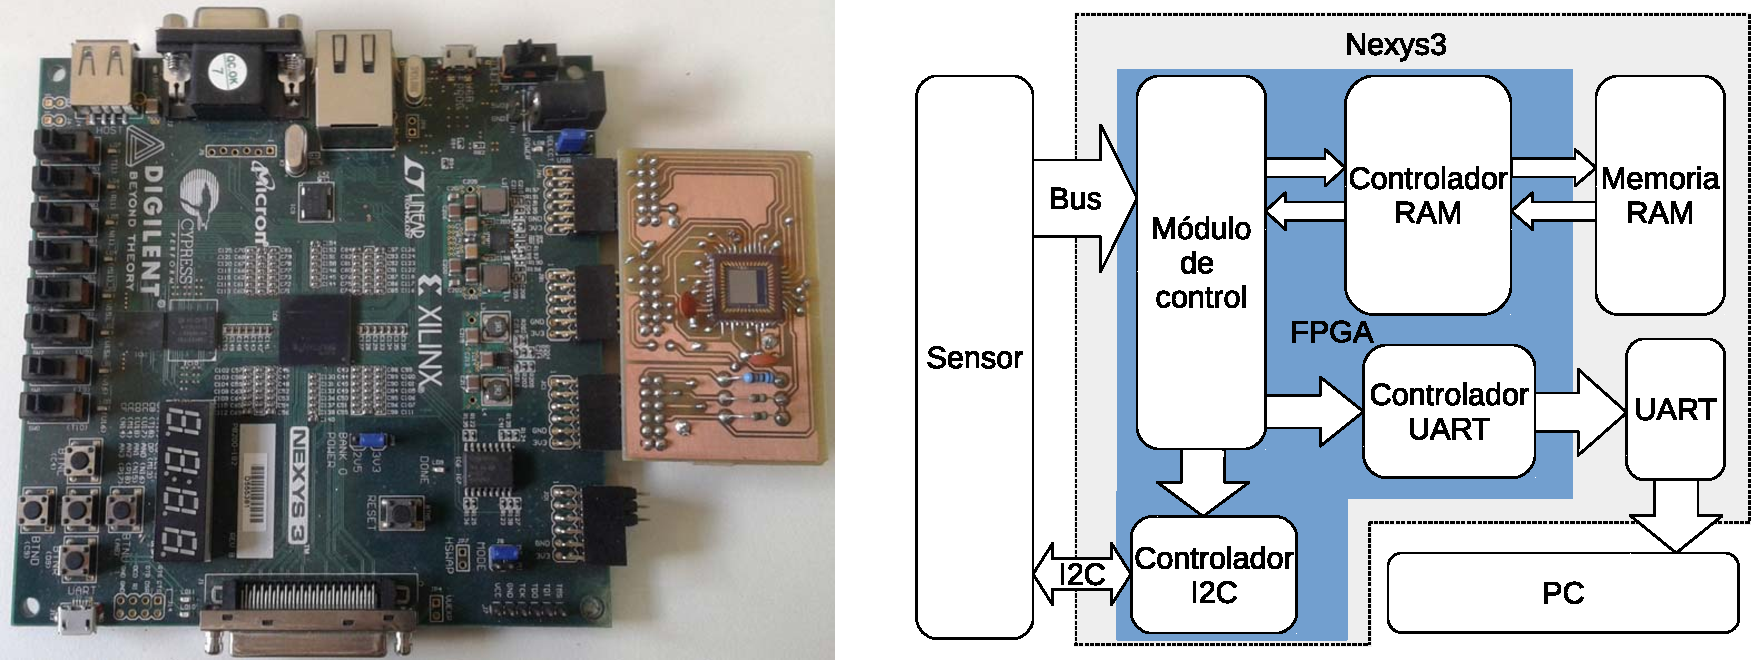
\includegraphics[width=0.9\paperwidth]{01motivacion}
	\end{frame}
	\begin{frame}{Agenda}
		\tableofcontents[hideallsubsections]
	\end{frame}
	\begin{frame}{Agenda}
		\tableofcontents[sections={1,2}]
	\end{frame}
	\begin{frame}{Agenda}
		\tableofcontents[sections={3,4}]
	\end{frame}
	\section{Introducción}
		\subsection{Motivación}
			\begin{frame}{La producción de información científica}
				\begin{itemize}
					\item Los avances en las escalas de integración de circuitos permiten desarrollar sensores que recolectan mayor volumen de datos.
					\item Los nuevos sensores necesitan nuevos circuitos adicionales que les permitan adquirir datos y controlar su funcionamiento.
					\item La utilización de FPGA es muy útil para sintetizar circuitos digitales.
					\item Los datos deben ser procesados para transformase en información.
					\item Los datos se deben transmitir desde los sistemas generadores a los sistemas procesadores.
				\end{itemize}
			\end{frame}
			%ACA me gustaría poner un frame donde se explique en forma gráfica lo de los sitemas procesadores y sistemas generadores
			\begin{frame}{La necesidad de una comunicación\\entre un FPGA y una PC}
				\begin{itemize}
					\item Las computadoras son herramientas muy útiles para procesar datos.
					\item Los FGPAs pueden operar a altas velocidades y utilizar puertos paralelos.
					\item Es de utilidad una comunicación entre las PCs y las aplicaciones que utilizan FPGA para la implementación de circuitos.
					\item USB es una opción robusta, con ancho de banda suficiente para transmitir imágenes e incorporada en cualquier PC moderna.
				\end{itemize}
			\end{frame}
		\subsection{Objetivos}
			\begin{frame}{Objetivos}
				\begin{itemize}
					\item Objetivo General
					\begin{itemize}
						\item Realizar una comunicación entre un FPGA y una PC mediante USB 2.0
					\end{itemize}
					\item Objetivos Particulares
					\begin{itemize}
						\item Comprender el funcionamiento del kit de desarrollo CY3684 y el framework provisto por Cypress.
						\item Configurar el chip CY7C68014A, incorporado en el kit de desarrollo anterior.
						\item Sintetizar un circuito en VHDL que sea capaz de interactuar con las memorias FIFO de la interfaz.
						\item Sintetizar circuitos de prueba para Test Bench.
						\item Validar el funcionamiento.
					\end{itemize}
				\end{itemize}
			\end{frame}
		\subsection{Bus Serial Universal}
			\begin{frame}{USB - Bus Serial Universal}
					El Bus Serial Universal o USB es un sistema de comunicación pensado, en su concepción original, para conectar periféricos a una PC.\\
					Los objetivos perseguidos por norma son:

				\begin{itemize}
					\item Conexión de telefonos a la PC.
					\item Facilidad de uso.
					\item Proveer un puerto de expansión para periféricos.
					\item<2-> \alert {Mayor rendimiento}
					\item<2-> \alert {Mayor ancho de banda}
%					\item Topológicamente, posee una estructura mestro-esclavo, en forma de árbol, donde el nodo principal es el Host, el resto de los nodos está implementado con Hubs y cada dispositivo es un esclavo.
%					\item Mecánicamente, posee dos pares de conductores, uno de alimentación ($V_{BUS}$ y GROUND) y otro de datos diferenciales(D+ y D-). Además posee diferentes tipos de fichas de conexión.
				\end{itemize}
				
				\only <2-> {La respuesta a esta demanda fue agregar una nueva velocidad de 480 Mbit/s.}
				
			\end{frame}
			\begin{frame}{USB - Topología}
				\centering
				\begin{itemize}
					\item \only<1> {Física} \only<2> {Lógica}
				\end{itemize}
				\only<1>{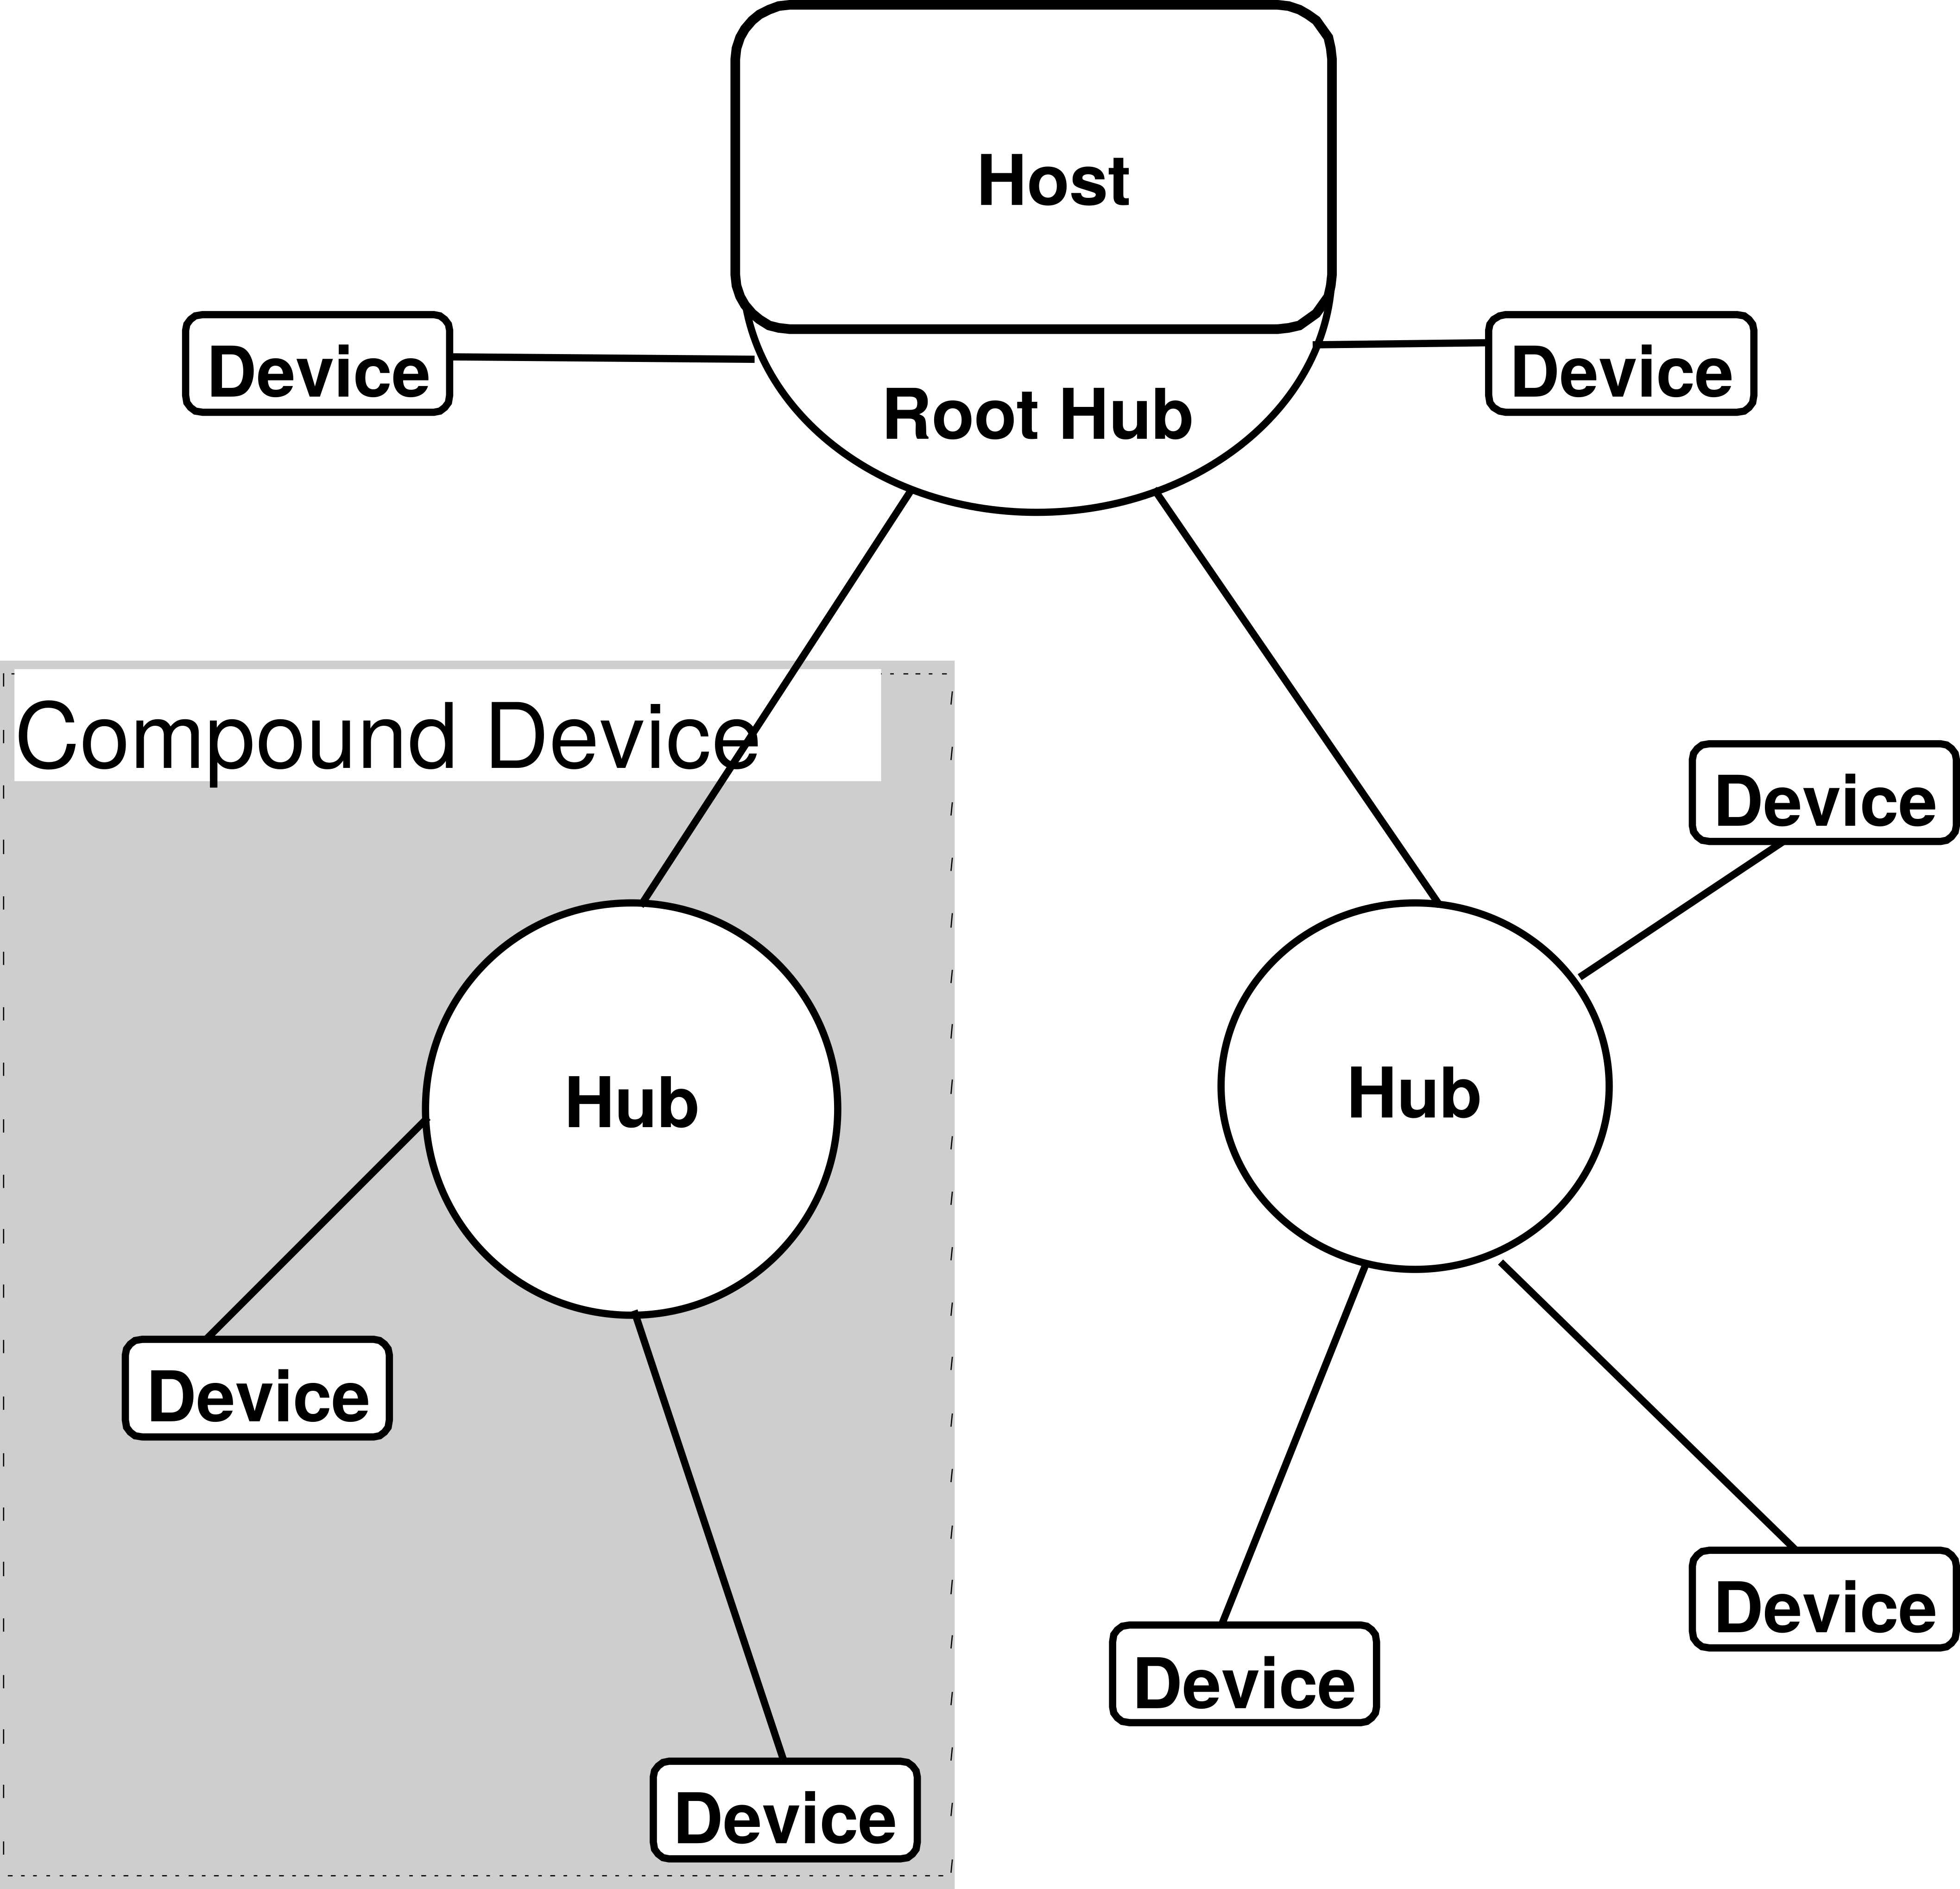
\includegraphics[width=0.6\textwidth]{topofisica.png}}
				\only<2>{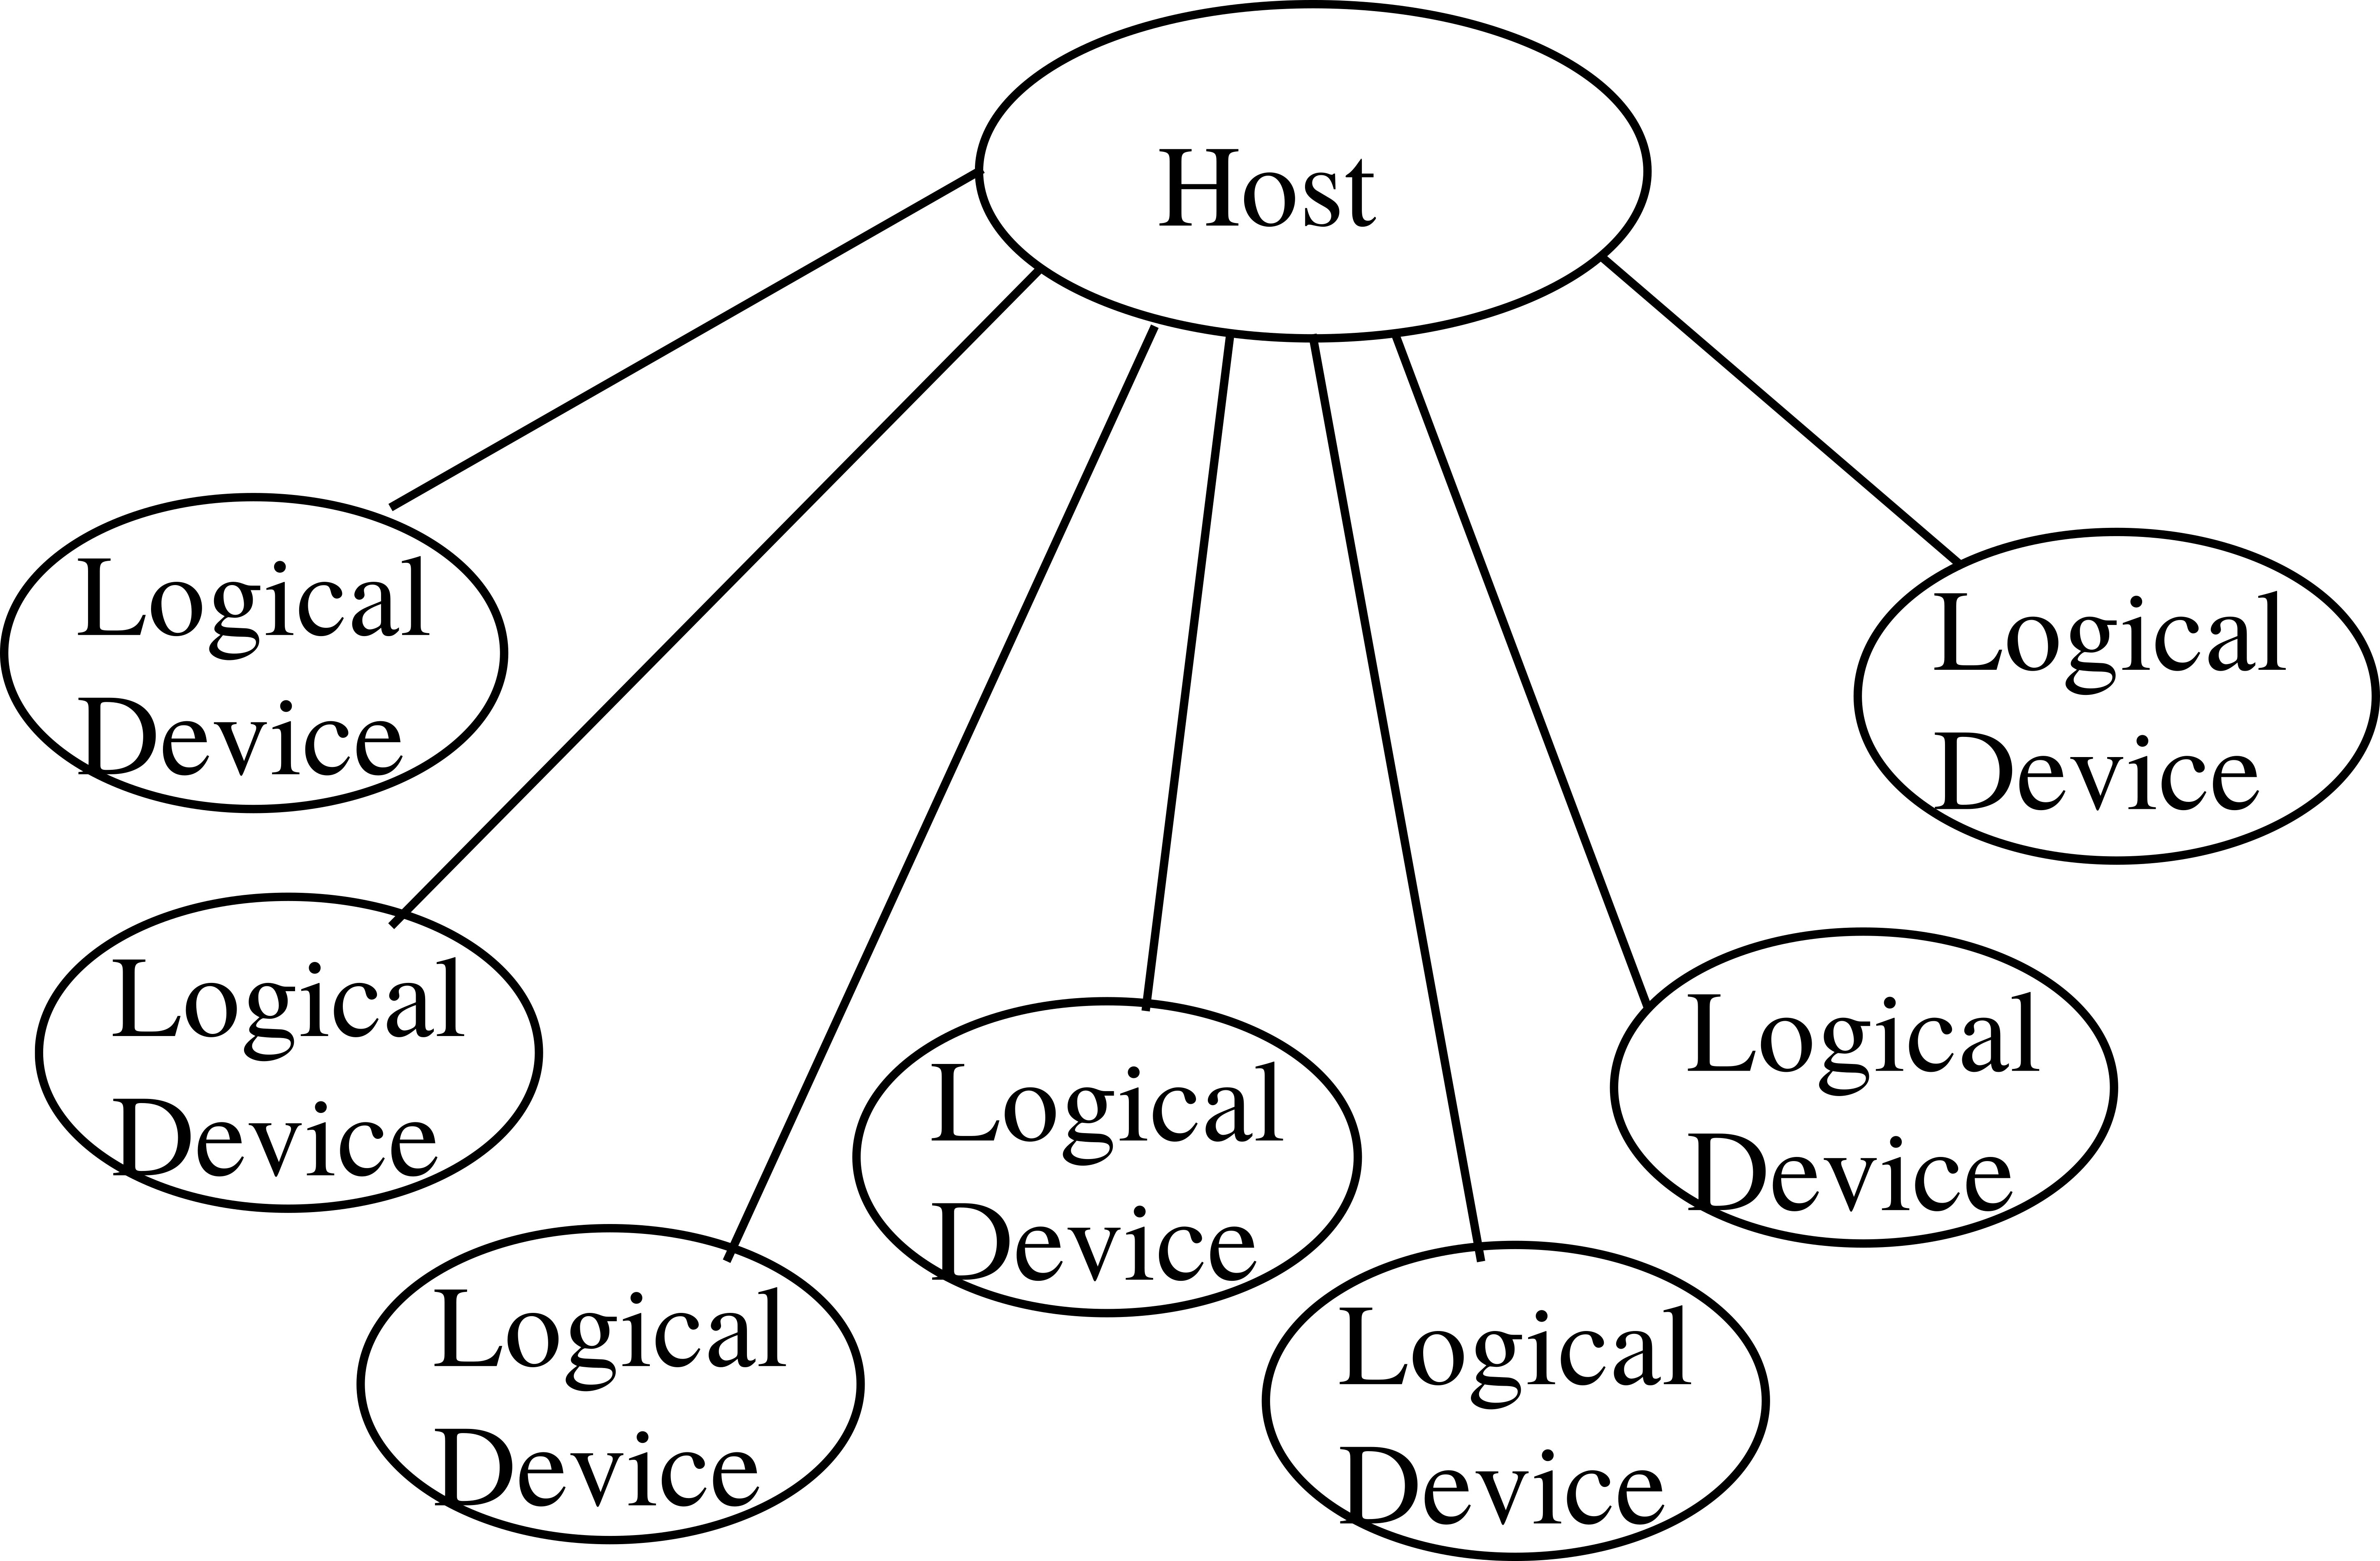
\includegraphics[width=0.8\textwidth]{topologica.png}}
			\end{frame}
			\begin{frame}{USB - Flujo de Datos}
				\centering
				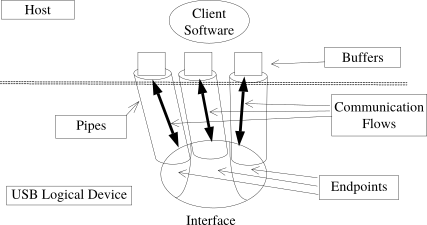
\includegraphics[width=0.8\textwidth]{complogicos.png}
			\end{frame}
			\begin{frame}{USB - Conexión mecánica}
				\begin{figure}
					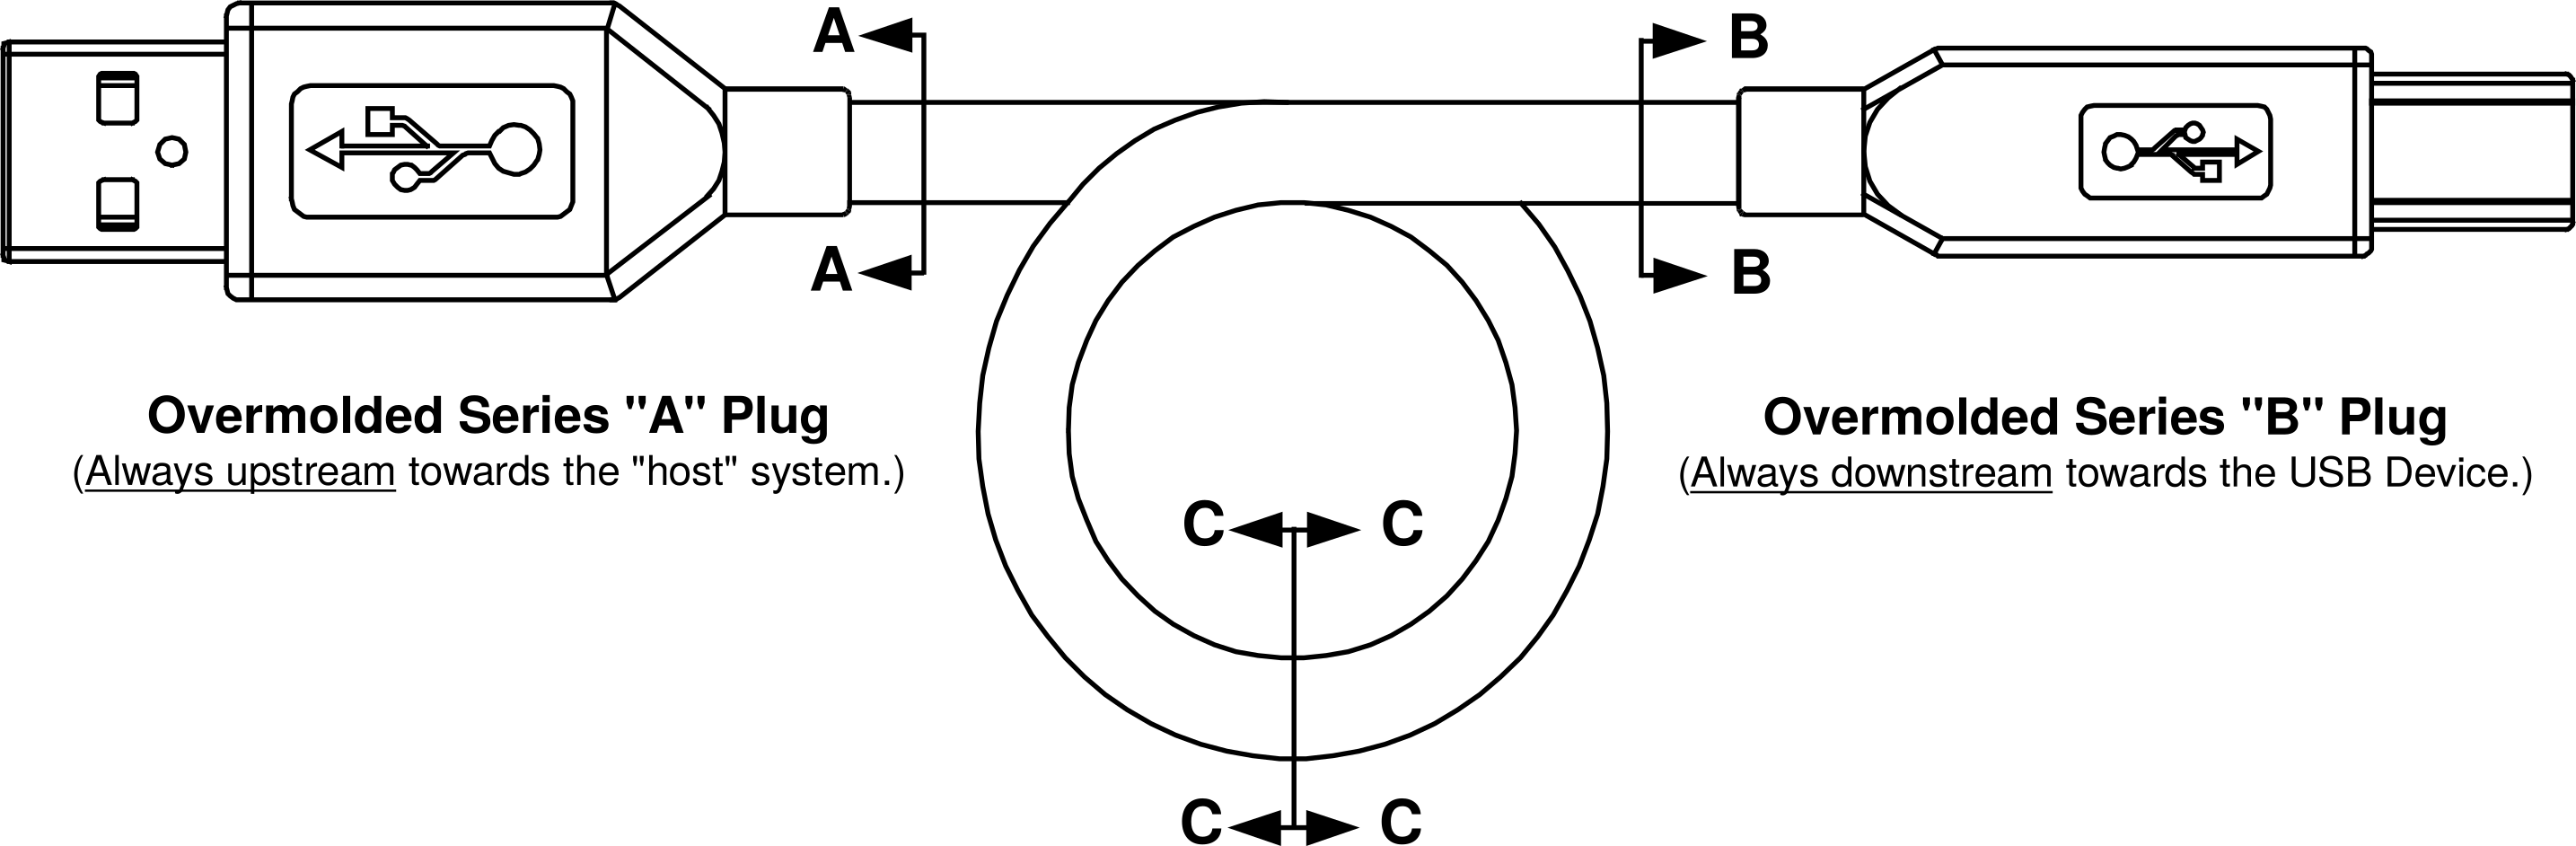
\includegraphics[width=.9\textwidth]{usbcableb.png}
				\end{figure}
			\end{frame}
			\begin{frame}{USB - Conexión mecánica}
				\begin{figure}
					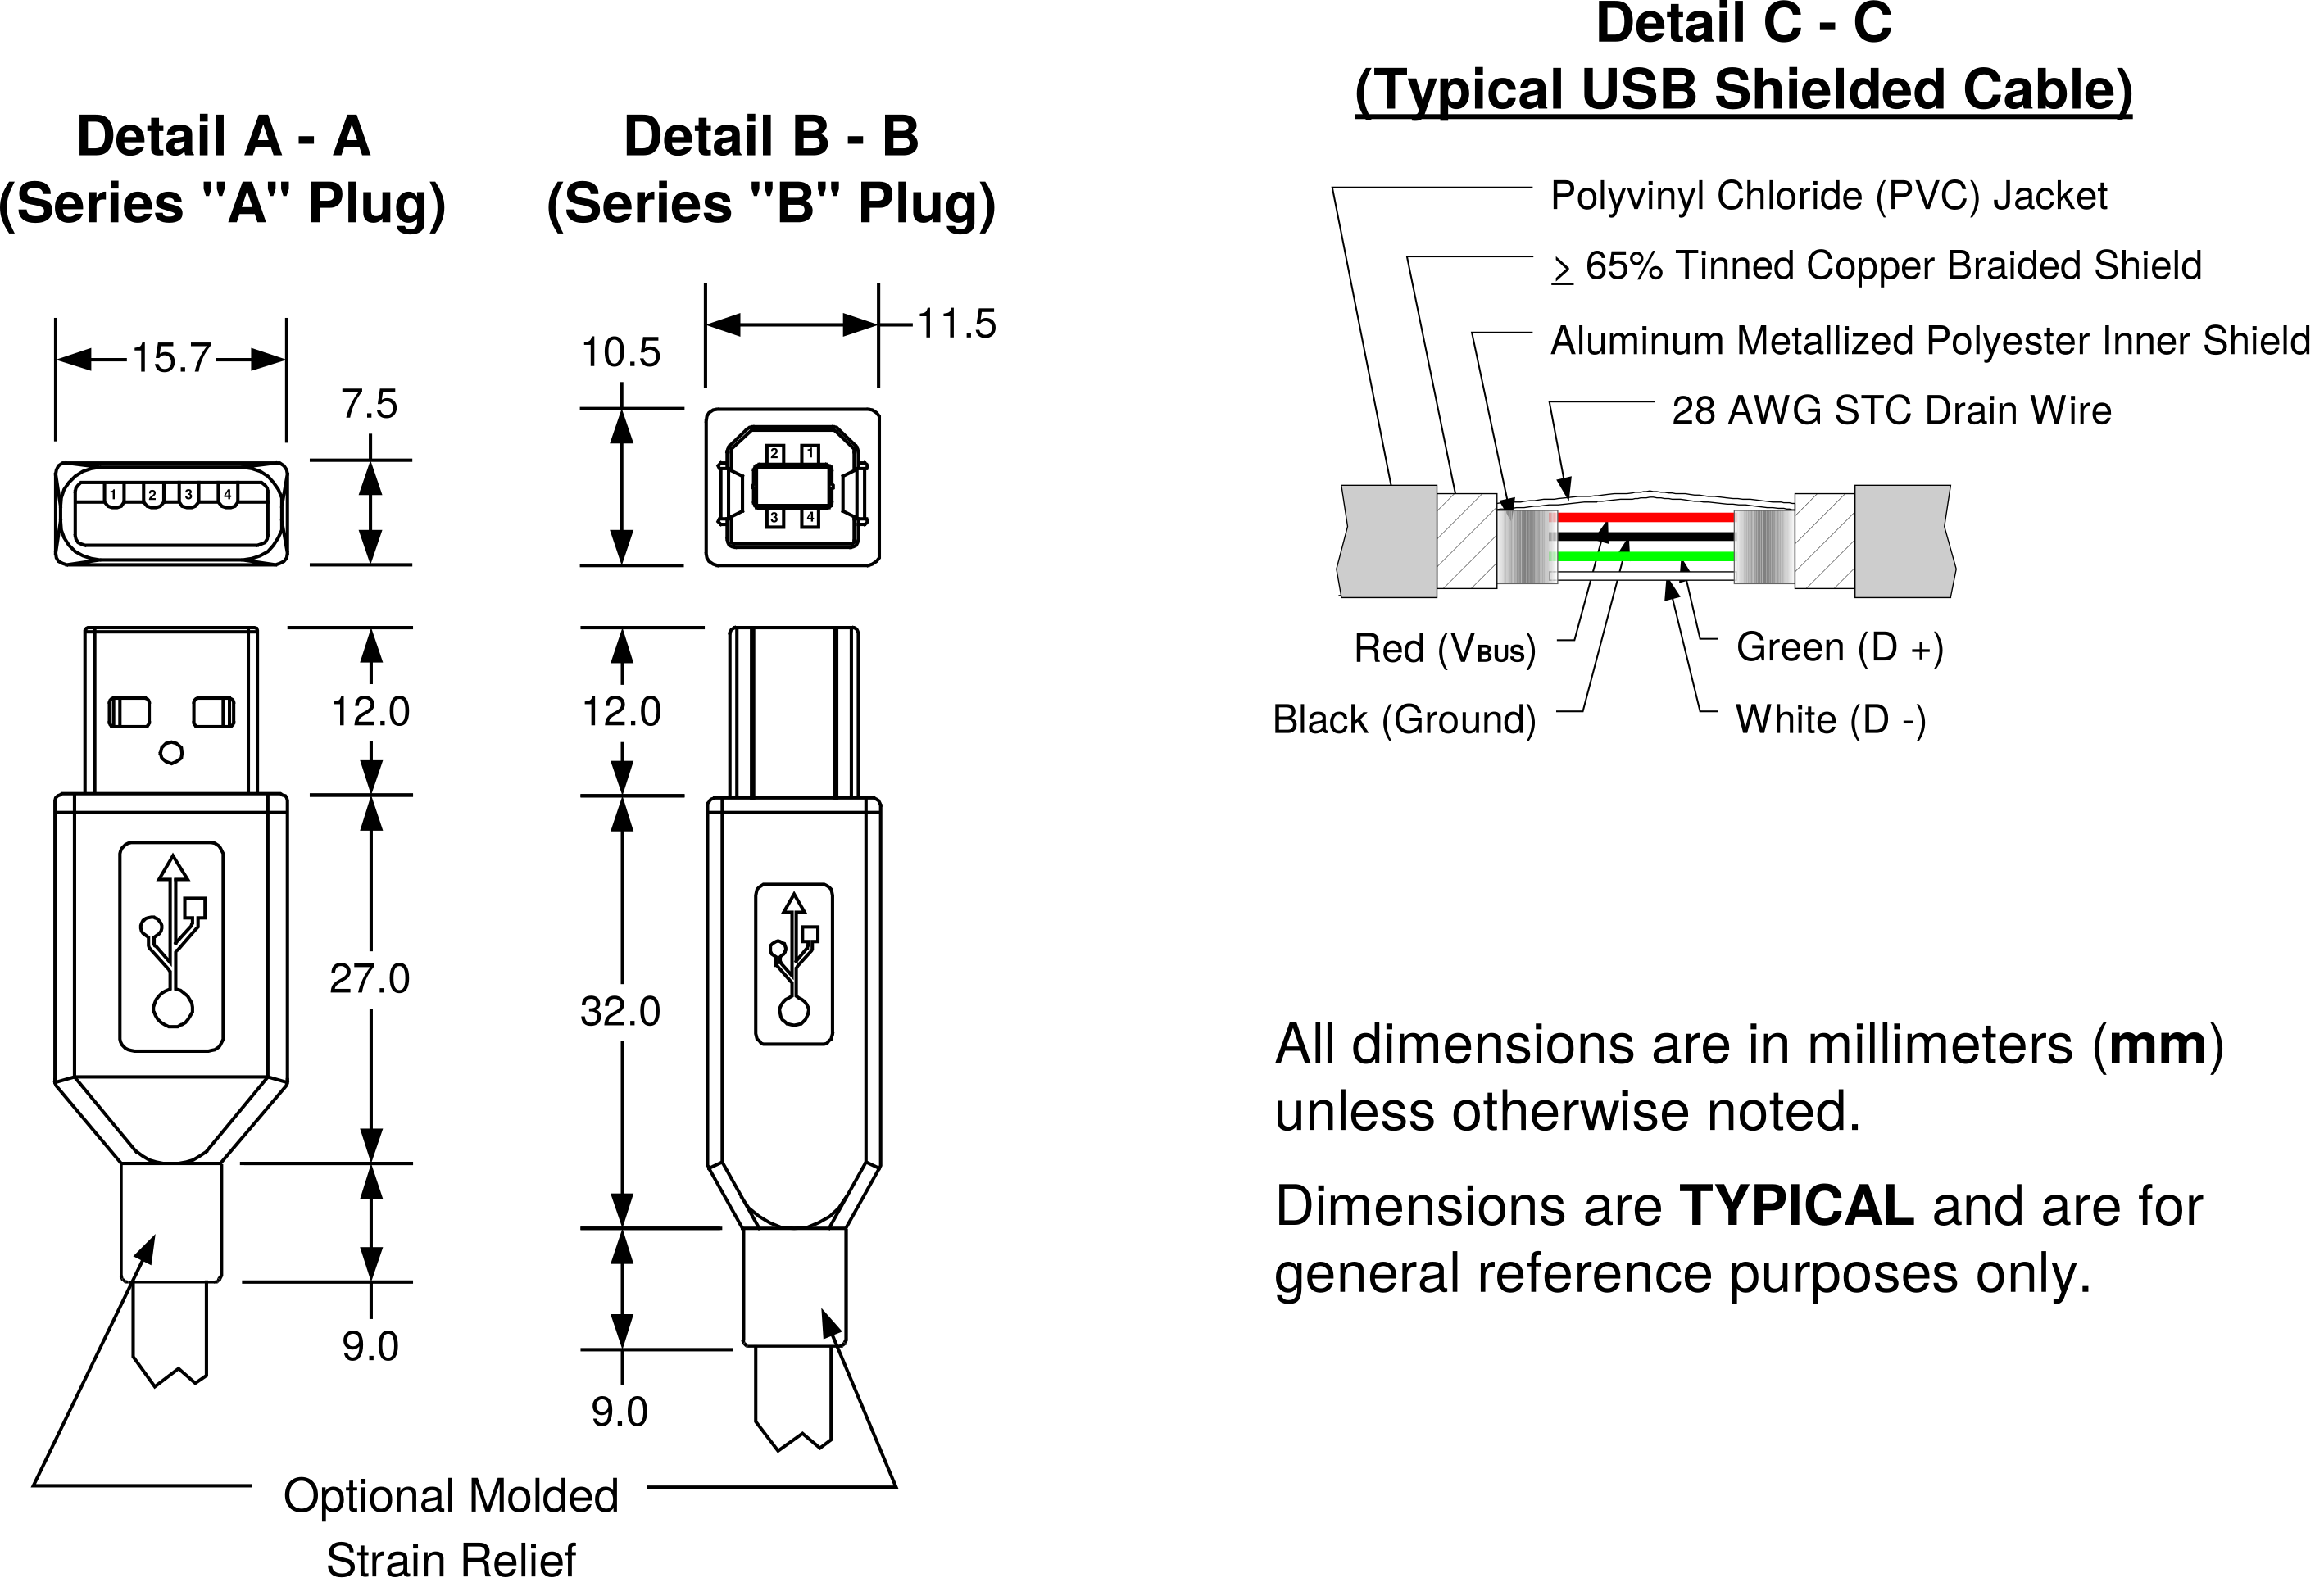
\includegraphics[width=0.9\textwidth]{usbcablea.png}
				\end{figure}
			\end{frame}
			\begin{frame}{USB - Especificaciones eléctricas}
				\begin{itemize}
					\item Existen 3 velocidades de señalización posibles:480 Mbit/s denominada high-speed, 12 Mbit/s para full-speed y 1.5 Mbit/s con low-speed.
					\item Se utiliza señal diferencial con un esquema de codificación NRZI (inversión de no retorno a zero).
					\item Los conductores de energía, $V_{BUS}$ y GROUND poseen \SI{5}{\volt} y \SI{0}{\volt} respectivamente.
					\item Los conductores de datos son diferenciales y están polarizados de forma tal que pueda ser identificada la velocidad de operación y la conexión/desconexión de dispositivos.
				\end{itemize}
			\end{frame}
			\begin{frame}{USB - Codificación NRZI}
				\begin{figure}
					\begin{tikzpicture}[scale=.6]
						\begin{scope}[transform shape,node distance=0.1,text width=20]
							\setcounter{wavecount}{0}
							\newwave{Data}
								\bit{0}{1}
								\bit{1}{2}
								\bit{0}{1}
								\bit{1}{1}
								\bit{0}{1}
								\bit{1}{1}
								\bit{0}{3}
								\bit{1}{1}
								\bit{0}{2}
								\bit{1}{2}
								\bit{0}{1}
							\newwave{NRZI - J}
								\bit{0}{3}
								\bit{1}{2}
								\bit{0}{2}
								\bit{1}{1}
								\bit{0}{1}
								\bit{1}{2}
								\bit{0}{1}
								\bit{1}{3}
								\bit{0}{1}
							\newwave{NRZI - K}
								\bit{1}{3}
								\bit{0}{2}
								\bit{1}{2}
								\bit{0}{1}
								\bit{1}{1}
								\bit{0}{2}
								\bit{1}{1}
								\bit{0}{3}
								\bit{1}{1}
						\end{scope}
						\begin{scope}[on background layer]
							\foreach \x in {1,2,...,16}{
								\draw[dashed,black!20] (\x.3,0) -- (\x.3,\value{wavecount}+1);}
						\end{scope}
					\end{tikzpicture}
				\end{figure}
			\end{frame}
%			\begin{frame}{USB - Bus Serial Universal}
%				\begin{itemize}
%					\item Lógicamente, cada dispositivo es visto desde el Host como un extremo.
%					\item Cada extremo posee un ``tubo'' de comunicación unidireccional y una dirección única.
%					\item Cada ``tubo'' tiene asignado en el Host un buffer específico.
%					\item Cada extremo tiene una única forma de comunicación con el Host, con su forma de acceso al bus y su determinada cuota de ancho de banda permitida.
%				\end{itemize}
%			\end{frame}
			\begin{frame}{USB - Tipo de Transferencias}
					Existen 4 tipos de transferencia los cuales difieren en cómo es transmitida la información, la dirección que posee, el tamaño máximo, acceso al bus, tiempos de latencia, manejo de errores y la secuencia de requerimiento de datos
				\begin{itemize}
					\item Transferencias de Control
					\item Transferencias de Interrupción
					\item Transferencias de Bultos
					\item Transferencias Isocrónicas
				\end{itemize}
				%AQUI me quedé
			\end{frame}
	\section{Implementación}
		\subsection{Arquitectura del sistema}
			\begin{frame}{Arquitectura del sistema propuesto}
				
			\end{frame}
		\subsection{Configuración del puente}
			\begin{frame}{Firmware de configuración de la interfaz}
				
			\end{frame}
		\subsection{Circuito sintetizado}
			\begin{frame}{Interfaz puente - FPGA}
				
			\end{frame}
		\subsection{Circuito de interconexión}
			\begin{frame}{Circuito de interconexión}
				\begin{itemize}
					\item Versión 1
					\item Versión 2
					\item Version 3
				\end{itemize}
			\end{frame}
	\section{Evaluación y validación}
		\subsection{Test benchs de VHDL}
			\begin{frame}{Test Bench}
				
			\end{frame}
		\subsection{Depuración de firmware del puente}
			\begin{frame}{Debug Cypress}
				
			\end{frame}
		\subsection{Biblioteca de PC}
			\begin{frame}{\texttt{libusb-1.0}}
				
			\end{frame}
		\subsection{Programas de prueba}
			\begin{frame}{Esquemas de prueba}
				
			\end{frame}
		\subsection{Elementos de VHDL utilizados para depuración}
			\begin{frame}{Flip-Flop para eco}
				
			\end{frame}
			\begin{frame}{ROM con patrón de repetición infinita}
				
			\end{frame}
	\section{Resultados y conclusiones}
		\subsection{Robustez}
			\begin{frame}{Resultados de la prueba de robustez\\de la comunicación}
				
			\end{frame}
		\subsection{Tasa máxima de Transferencia}
			\begin{frame}{Resultados de la prueba de máxima transferéncia de datos}
				TODO
			\end{frame}
		\subsection{Trabajo futuro}
			\begin{frame}{Lo que falta...}
				
			\end{frame}
			\begin{frame}{Consultas}
				
			\end{frame}
			\begin{frame}[c]
				\centering
				\alert {Muchas gracias}
			\end{frame}
			
			\begin{frame}{Material Adicional}
				\centering
				Respaldo y cosas que no entren
			\end{frame}
\end{document}